\documentclass{article}
\usepackage{listings}
\usepackage{graphicx}
\usepackage{xcolor}

% Farben für den Code-Block definieren
\lstset{
    basicstyle=\ttfamily\footnotesize,
    keywordstyle=\color{blue},
    commentstyle=\color{gray},
    stringstyle=\color{red},
    frame=single,
    breaklines=true,
    numbers=left,
    numberstyle=\tiny\color{gray},
}

\title{Erste Schritte mit YOLOv5}
\author{}
\date{}

\begin{document}
\maketitle

\section*{Software-Abhängigkeiten installieren}

\subsection*{1. Jetson-Inferenz-Toolkit}
NVIDIA bietet das \textbf{Jetson Inference}-Projekt an, das vortrainierte Modelle und Beispielanwendungen für Objekterkennung, Klassifikation und Segmentierung enthält.

\begin{lstlisting}[language=bash]
git clone --recursive https://github.com/dusty-nv/jetson-inference
# Falls der obige Befehl nicht funktioniert:
git clone --recursive --depth 1 https://github.com/dusty-nv/jetson-inference
\end{lstlisting}

Wechslen Sie ins Verzeichnis:
\begin{lstlisting}[language=bash]
cd jetson-inference
\end{lstlisting}

Überprüfen Sie den Status des Repositories:
\begin{lstlisting}[language=bash]
git status
\end{lstlisting}

\subsection*{2. Build-Prozess}
Erstellen Sie das Projektverzeichnis und bauen Sie das Projekt:
\begin{lstlisting}[language=bash]
cd jetson-inference
mkdir build
cd build
cmake ../
make -j$(nproc)
sudo make install
\end{lstlisting}

\subsection*{3. Python-Bibliotheken installieren}
Je nach Projekt können folgende Python-Bibliotheken installiert werden:

\begin{lstlisting}[language=bash]
sudo apt-get update
sudo apt-get install python3-pip
pip3 install numpy opencv-python matplotlib
pip3 install torch torchvision --extra-index-url https://download.pytorch.org/whl/cu118
\end{lstlisting}

\subsection*{4. YOLOv5/YOLONano verwenden}
Laden Sie YOLOv5 herunter und installieren Sie die Abhängigkeiten:
\begin{lstlisting}[language=bash]
git clone https://github.com/ultralytics/yolov5 
cd yolov5
pip3 install -r requirements.txt
python3 detect.py --source 0 
\end{lstlisting}
% python3 detect.py --source 0  Für Kamera-Input

Falls ein Fehler wie folgend auftritt: 
\textit{ValueError: numpy.dtype size changed, may indicate binary incompatibility. 
Expected 96 from C header, got 88 from PyObject}

Nutze diesen Befehl zur Behebung:
\begin{lstlisting}[language=bash]
pip3 install --upgrade --force-reinstall -r requirements.txt
\end{lstlisting}
Wiederholen Sie die vorherigen Schritte.

% \subsection*{5. Kamera-Setup und Videoaufnahme}
% Überprüfe, ob die Kamera funktioniert:
% \begin{lstlisting}[language=bash]
% gst-launch-1.0 nvarguscamerasrc ! nvoverlaysink
% \end{lstlisting}

% Für USB-Kameras:
% \begin{lstlisting}[language=bash]
% python3 detectnet-camera.py
% \end{lstlisting}

% \subsection*{6. Optimierung mit TensorRT}
% Beschleunige dein Modell mit \textbf{TensorRT}, um die Latenz zu reduzieren:
% \begin{lstlisting}[language=bash]
% sudo apt-get install tensorrt
% python3 trt_infer.py --engine model.trt
% \end{lstlisting}
\section{YOLOv5 startet}
die Kamera wird geöffnet und der Modell fängt an Objekte zu erkennen.
Dabei sieht der Terminal wie folgendes aus: 
\begin{figure}[h!]
    \centering
    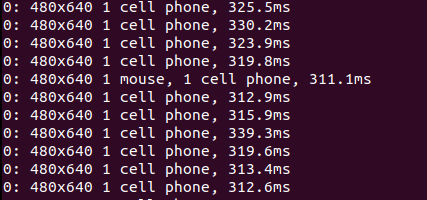
\includegraphics[width=0.8\textwidth]{Bilder/terminalErgebnisse.png}
\end{figure}

\clearpage
\section{Erkennungsbeispiele:}
Im folgenden sind ein paar Gegenstände, die mit YOLOv5 erkennt wurden.
\subsection{Handy}
Erkennung von Handy: 

\begin{center}
    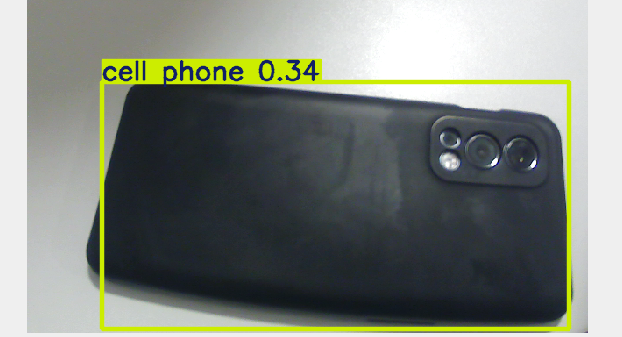
\includegraphics[width=0.8\textwidth]{Bilder/handyErkennung.png}
\end{center}

\subsection{Maus}
Erkeenung von Maus:

\begin{center}
    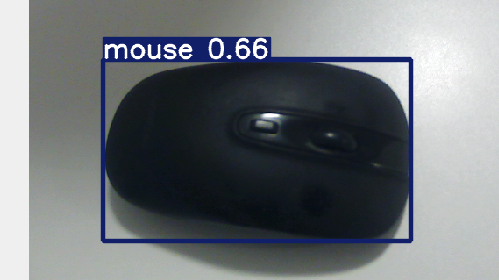
\includegraphics[width=0.8\textwidth]{Bilder/mausErkennung.png}
\end{center}

\subsection{Tastatur}
Erkennung von Tastatur: 

\begin{center}
    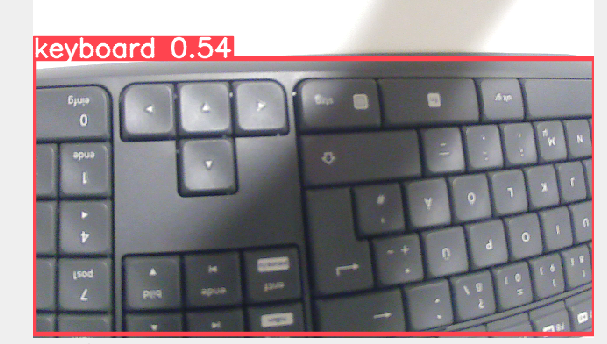
\includegraphics[width=0.8\textwidth]{Bilder/tastaturErkennung.png}
\end{center}
\end{document}
